\documentclass[11pt,a4paper]{article}

% ------ PACKAGES ------

\usepackage[utf8]{inputenc}%encodage en utf8
\usepackage[english]{babel} %permet caractères français
\usepackage[T1]{fontenc} %permet cararct spéciaux
\usepackage{hyperref}  %liens hypertextes

\usepackage{array}
\usepackage{float}
\usepackage{lscape}

\usepackage{amsmath,amsthm} %pour les maths
\usepackage{commath}
\usepackage{setspace}%pour avoir un inteligne de 1.5

\usepackage{multirow}  %Tableaux à plusieurs lignes

\usepackage{geometry}%réglages mise en page
\usepackage{fancyhdr}%for headers and footers
\pagestyle{fancy}
\usepackage{algorithm}
\usepackage{algorithmic}
\usepackage{optidef} %formules d'optimisation

\usepackage{parskip}

\newtheorem{theorem}{Theorem}
\newtheorem{defn}[theorem]{Definition}
\newtheorem{example}[theorem]{Example}
\newtheorem{remark}[theorem]{Remark}
\newtheorem{question}[theorem]{Question}

\newtheorem{lemma}[theorem]{Lemma}
\newtheorem{claim}[theorem]{Claim}
\newtheorem{prop}[theorem]{Proposition}
\newtheorem{corollary}[theorem]{Corollary}
\newtheorem{conjecture}[theorem]{Conjecture}

\newtheorem{hyp}[theorem]{Hypothesis}

\onehalfspacing   %interligne de 1.5

\renewcommand{\algorithmicrequire}{\textbf{Input:}}
\renewcommand{\algorithmicensure}{\textbf{Output:}}

% ------ ADD SUBSUBSECITONS ------
\setcounter{secnumdepth}{3}
\setcounter{tocdepth}{3}

% ------ PAGE LAYOUT ------
\geometry{
%a4paper
%body={170mm,260mm},
left=35mm, top=25mm,
bottom=25mm, right=25mm
%headheight=10mm, headsep=10mm,
%footskip=10mm
}

% ---------- COMMAND SETTERS -----------

\newcommand{\HRule}{\rule{\linewidth}{0.5mm}} %newcommand for cover page

\begin{document}
\begin{titlepage}
\begin{center}

\textsc{\LARGE universit\'e libre de bruxelles}\\[2.5cm]

% Upper part of the page. The '~' is needed because \\
% only works if a paragraph has started.

\includegraphics[width=0.3\textwidth]{Images/ulblogo.jpg}~\\[1cm]

\textsc{\Large  TRAN-F501 \\[0.3cm] Internship - 201819 }\\[0.5cm]

% Title
\HRule \\[0.6cm]
{ \huge \bfseries Project:
A stochastic simulation system for protein aggregation \\[0.6cm] }

\HRule \\[2cm]

% Author and supervisor

\begin{center} \large
\emph{Supervisor:} \\
Tom \textsc{Lenaerts}\\


\emph{Author:}\\
Prateeba\textsc{ Ruggoo}\\
\end{center}

\vfill

% Bottom of the page
{\large \today}

\end{center}
\end{titlepage}


\tableofcontents \pagebreak

\section{Introduction}
Diseases like Alzheimer and Parkinson disease are the result of proteins aggregating into large fractal structures that hinder the cell function or even destroy them. Understanding how aggregates are formed and change over time is important to understand when they become harmful and how maybe treatments affect aggregate formation.

The goal of this Internship is to work on the implementation of a simulation system required to study aggregation between proteins. This work is performed in collaboration with the Switch lab in the KU Leuven, who have an extensive expertise in studying aggregation and related diseases.

\section{First 2 weeks (12th-23rd August)}
(Maybe add the administrative part, introduction to the team members and all...)
During the first two weeks of the intership, I researched the subject and mostly did a of state of the around the subject to have a baseline knowledge around the subject. !!!!!!!!!!!!!!! TO ADD MORE DETAILS !!!!!!!!!!!!!!!!!!!

\section{Third week (26th-31st August)}
Now having a basic understanding around the subject, I could refine my reasearch and focus on the specific papers discussing the problem in order to have a
deeper understanding of the theory before starting any kind of implementation.
!!!!!!!!!!!!!!! TO ADD MORE DETAILS !!!!!!!!!!!!!!!!!!!

\section{Fourth week (2nd-6th September)}
The goal of this week was : To implement a simple prototype (in python for now) of an exact numerical simulation method to simulate trajectories of discrete, stochastic systems.

\subsection{Step 1 : Mathematical Descriptions of Chemical Processes}
A coupled system of chemical reactions of the form :
$X_{1} + X_{2} \rightarrow X_{3} + ...$ states that one molecule from substance $X_{1}$ reacts with one molecule of substance $X_{2}$ to give one molecule of substance $X_{3}$

\subsubsection{Hypothesis :}
The solution is well mixed $\rightarrow$ nonreactive collisions occur far more than reactive collisions $\rightarrow$ fast dynamics of motion can be neglected $\rightarrow$ Can use the number of each kind of molecule to represent the system.

\begin{theorem}
The probability that a certain reaction $\mu$ will take place in the next instant of time $dt$ is given by $a_{\mu}dt + o(dt)$, where $a_{\mu}$ is independent of $dt$.
\end{theorem}

\subsection{The stochastic framework}
\begin{enumerate}
  \item We have a set of reactions
    \begin{gather}
      {A + B \rightarrow^{k_1} C}  \\
      {B + C \rightarrow^{k_2} D}  \\
      {D + E \rightarrow^{k_3} E + F} \\
      {F \rightarrow^{k_4} D + G} \\
      {E + G \rightarrow^{k_5} A}
    \end{gather}
  \item The propensities of the reactions are given by $k_{1}, k_{2}, ... k_{5}$
  \item The probability that a given molecule $A$ reacts with a given molecule $B$ in a small time $dt$ is $k_{1}dt + o(dt)$.
\end{enumerate}

\subsubsection{Gillespie's stochastic framework of chemical kinetics}
The principle task is to develop a method for simulation the time evolution of the $N$ quantities $\{X_{i}\}$, knowing only their initial values $\{X_{i}^{(0)}\}$, the form of the $M$ reactions $\{R_{\mu}\}$ and the values of the reaction parameters $\{c_{\mu}\}$.

\begin{defn}{Problem definition : }
We are given a volume $V$ containing molecules of $N$ chemically active species $S_{i}(i = 1, \dots, N)$. Let $X_{i} \equiv$ current number of molecules of chemical species $S_{i} \in V, (i = 1, 2, \dots, N)$ and let $R_{\mu} (\mu = 1, \dots, M)$ be the chemical reactions in which the species $S_{i}$ can participate where each reaction $R_{\mu}$ is characterized by a numerical reaction parameter $c_{\mu}$.
\end{defn}
\begin{defn}{Type of reactions}
\begin{gather}
  {* \rightarrow reaction products}  \\
  {S_{j} \rightarrow reaction products} \\
  {S_{j} + S_{k} \rightarrow reaction products}\\
  {2S_{j} \rightarrow reaction products} \\
  {S_{i} + S_{j} + S_{k} \rightarrow reaction products}\\
  {S_{j} + 2S_{k} \rightarrow reaction products} \\
  {3S_{j} \rightarrow reaction products}
\end{gather}
\end{defn}

\begin{hyp}{Fundamental Hypothesis}
The reaction parameter $c_{\mu}$ can be defined as follows :
\begin{defn} $c_{\mu} \delta t \equiv $ avarage probability that a particular combination of $R_{\mu}$ reactant molecules will react accordingly in the next time interval $\delta t$ (first order)
\end{defn}
\end{hyp}

!!!!!!!!!!!!!!!!!!!!!! TO DO : FINISH THE DETAILS AND EXPLANATION OF EACH FORMULA !!!!!!!!!!!!!!!!!!!!!!!!!!!!!!

\begin{defn}State of the system is defined by the number of molecules of each species and changes discretely whenever one of the reactions is executed. The probability that a certain reaction $\mu$ will take place in the nest instant of time is given by $a_{\mu}dt + o(dt)$

  \begin{example} Let $S$ be the set of states $i.e$ $S = (\#A, \#B, \#C, \#D, \#E, \#F, \#G)$, $S$ will change to $S^{'} = (\#A-1, \#B-1, \#C+1, \#D, \#E, \#F, \#G)$ if Reaction $1$ is executed. The probability of this occurence is given by :
  $P(S^{'}, t + dt|S,t) = a_{1}dt + o(dt)$
  \end{example}

\end{defn}

\begin{figure}[!h]
\centering
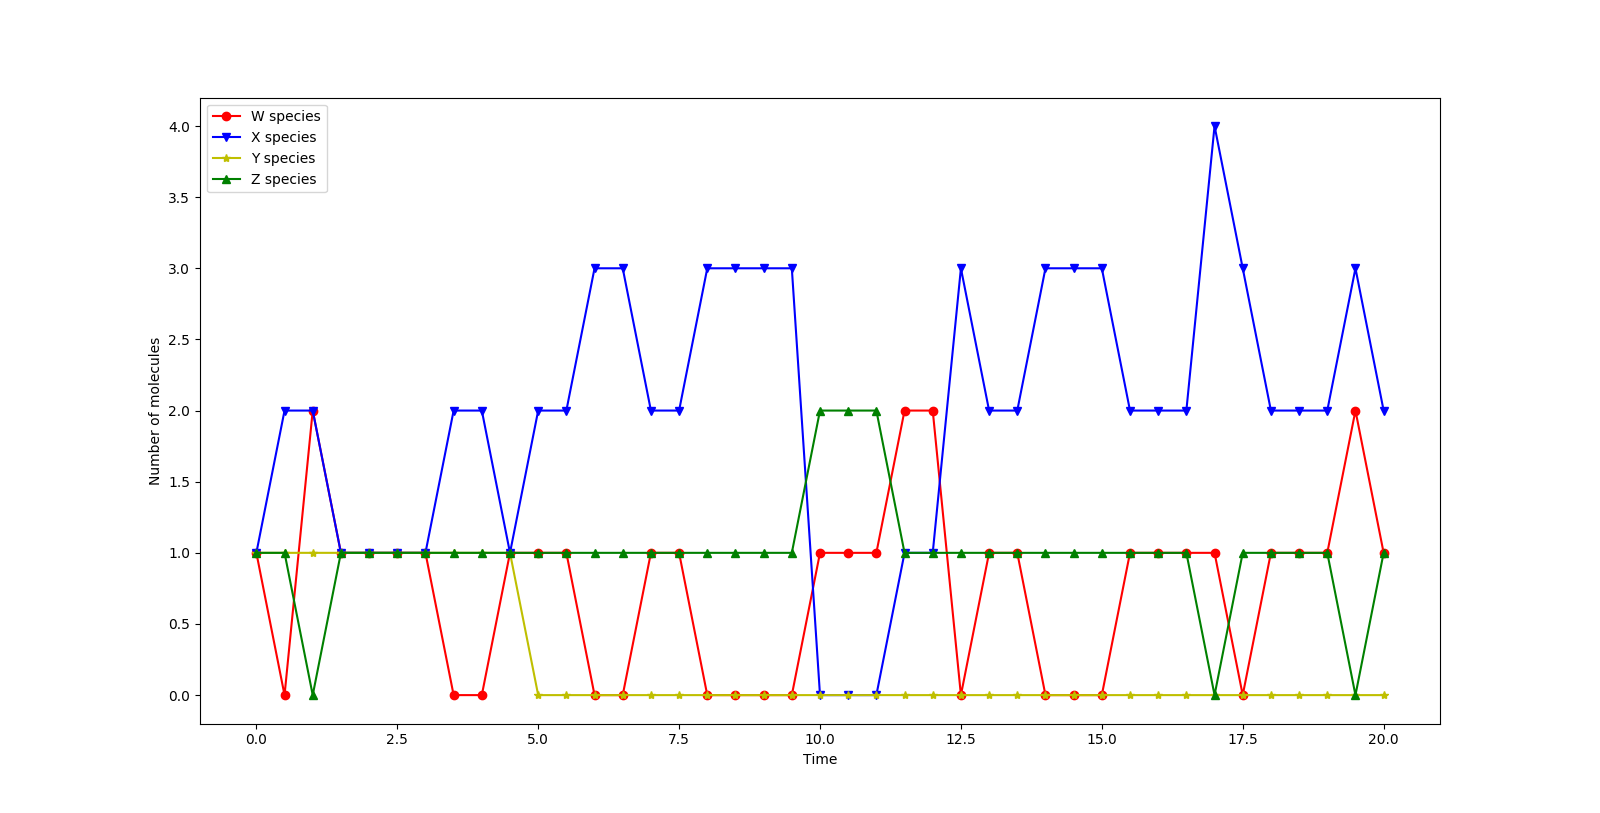
\includegraphics[width=1\textwidth]{Images/Figure_1.png}
\caption{The x-axis denotes the dataset used and the y-axis denotes the computation time}
\label{fig:barplot random 50}
\end{figure}

\section{Gillespie's algorithm}
    \begin{algorithm}[!h]                     % enter the algorithm environment
    \caption{Gillespie's algorithm}           % give the algorithm a caption
    \begin{algorithmic}                       % enter the algorithmic environment

    \REQUIRE
    \ENSURE

    \WHILE{!$($number of reactants = 0 || simulation time exceeded $)$ }
    \STATE 1. Initialization: Initialize the number of molecules in the system, reaction constants, and random number generators.
    \STATE 2. Monte Carlo step: Generate random numbers to determine the next reaction to occur as well as the time interval. The probability of a given reaction to be chosen is proportional to the number of substrate molecules, the time interval is exponentially distributed with mean $1/R_{TOT}$
    \STATE 3. Update: Increase the time by the randomly generated time in Step 2. Update the molecule count based on the reaction that occurred.

    \ENDWHILE
    \end{algorithmic}
    \end{algorithm}

\section{Initial values}

\begin{enumerate}
  \item $n_{A} = n_{B} = 10$
  \item $n_{AB} = 0 $
  \item $t = 0$
  \item $k_{D} = 2 $
  \item $k_{B} = 1 $

\end{enumerate}

\section{Gillespie's algorithm : Simple example}

\subsection{Reaction Rates}
  \begin{enumerate}
    \item If we consider two types of mocules : $A$ and $B$, two types of reaction can happen.
    \begin{enumerate}
      \item $A$ and $B$ bind together to form $AB$ dimer.
      \item $AB$ dimers dissociates into an $A$ and a $B$ molecule.
    \end{enumerate}
    \item let $k_D$ be the reaction rate for a $AB$ dimer formation.
    \item let $k_B$ be the reaction rate for a $AB$ dimer deformation.
    \item So at a time $t$, the total reaction rate $ = k_D \cdot$ number of type $A$ molecules $\cdot$number of type $B$ molecules$ + k_B\cdot$ number of $AB$ dimers $	\Rightarrow R_{TOT} = k_{D}n_{A}n_{B} + k_{B}n_{AB}$.
  \end{enumerate}

\subsection{Time evolution}
Two steps to perform to advance forward in time.
\begin{enumerate}
  \item Calculate the time to the next reaction.
    \begin{enumerate}
      \item Determining reaction concern predicting how much time we need to wait before a reaction happens. Since this time is unknown, it is often appropriate to think of it as a random variable having an exponential distribution.
      \item Here the next reaction time is a random number drawn from exponential distribution function with mean $1/R_{TOT}$.
      \item Thus we move from time $t$ to $\delta t$
    \end{enumerate}

  \item Determine the next reaction among the possible reactions.
  \begin{enumerate}
    \item $P(A + B  \rightarrow AB) = k_{D}n_{A}n_{B} / R_{TOT} $
    \item $P(AB  \rightarrow A + B) = 1 - (k_{D}n_{A}n_{B} / R_{TOT}) $
  \end{enumerate}
  So with these two probabilities we either :
  \begin{enumerate}
  \item Form a dimer by reducing $n_{A}$ and $n_{B}$ by one and increase $n_{AB}$ by one.
  \item Or dissociate an $AB$ dimer by adding one to $n_{A}$ and $n_{B}$ and minus one to $n_{AB}$
  \end{enumerate}
\end{enumerate}
The Gillespie algorithm repeats these two steps as many times as needed to simulate the system for as many reactions as we want.

\section{Conclusion}

\newpage
\bibliographystyle{alpha}
\bibliography{combinatorial}


\end{document}
